\documentclass[11pt,a4paper]{article}

% Packages
\usepackage[utf8]{inputenc}
\usepackage[T1]{fontenc}
\usepackage{graphicx}
\usepackage{hyperref}

% Document information
\title{Rede Neural para IR Spectra Documentação}
\author{Ian Bezerra}
\date{\today}

\begin{document}

\maketitle

\begin{abstract}
    Usando redes Neurais para classificar funcoes organicas presentes em um espectro de IR.
\end{abstract}

\section{Introdução}
Inicialmente fizemos uma construção de uma rede neural onde classificamos espectros de XRD em moléculas inorgânicas na área da cristalografia, este projeto foi bem sucedido, pela simplicidade do problema abordado, que era de classificação, e o fato de espectros de XRD apresentarem menos variações, conseguimos chegar a grandes precisões com uma rede neural relativamente simples. Com isso seguimos para um problema mais complexo, em uma área onde a complexidade de espectro é muito maior.

A área agora é a química orgânica, vamos para uma simples introdução do problema e o que uma rede neural faria, para depois ampliar a especificações do problema.

\begin{figure}[h]
    \centering
    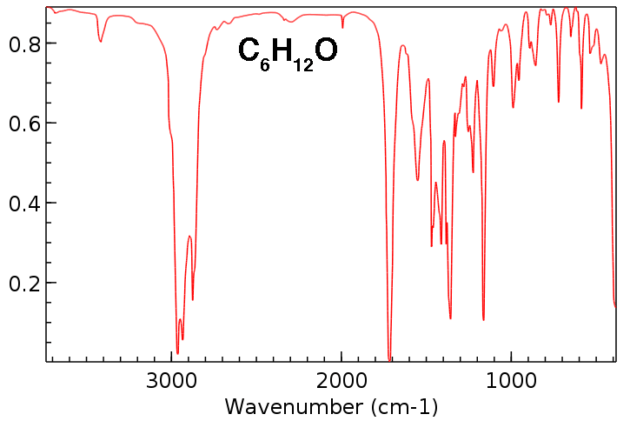
\includegraphics[width=0.8\textwidth]{Images/spec.png}
    \caption{Espectro de IR}
    \label{fig:ir_spectrum}
\end{figure}

Espectroscopia de infravermelho é uma técnica analítica versátil na química orgânica e outras ciências. Utiliza ondas eletromagnéticas infravermelhas para interagir com ligações químicas em moléculas. A absorção de energia em frequências específicas cria um espectro único, funcionando como "impressão digital" molecular. Permite identificar grupos funcionais, determinar estruturas e analisar composições. É não destrutiva, aplicável a diversos estados da matéria, sendo essencial em pesquisa e indústria.

\begin{figure}[h]
    \centering
    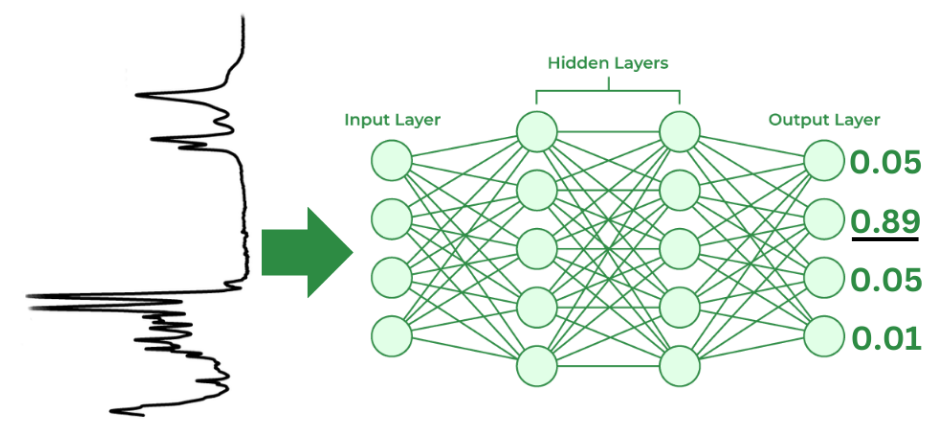
\includegraphics[width=0.8\textwidth]{Images/NN2.png}
    \caption{Rede Neural de Classificacao(Rede nao condiz com a arquitetura usada)}
    \label{fig:ir_spectrum}
\end{figure}

Em uma implementação de classificação usamos o espectro como input e usamos uma rede neural para gerar um output na ultima camada uma distribuição de probabilidade em cima de um dicionário de moléculas conhecidas. Assim, assumimos que a molécula com maior probabilidade é a escolha da rede neural, também é importante criar um threshold onde se à maior probabilidade for menor que este threshold, então dizemos que a rede neural “não tem certeza”. Isso pode acontecer quando colocamos como input uma molécula que não estava nos dados usados para treinar e dessa forma a rede neural não aprendeu a classificá-la.


\section{Classificacao funcoes organicas em espectros de IR}

Quando fazemos a classificação da molécula, observamos o espectro como sua impressão digital, achando similaridades entre o espectro de input e as digitais únicas das moléculas aprendidas, onde a rede neural aprende padrões únicos de cada molécula e ativa neurônios quando identifica cada padrão, subindo assim a ativação do neurônio final que representa a probabilidade da amostra ser a respectiva molécula deste índice no dicionário.

Diferentemente do problema de classificação de moléculas, a classificação de funções orgânicas dentro do espectro do IR não busca aprender a impressão digital de cada molécula, mas sim os padrões criados pela presença de uma função orgânica específica dentro de um espectro de IR. Desta forma, seria possível fornecer o input de um espectro de IR de uma molécula nunca antes vista pela rede neural, e reconhecer os padrões das funções orgânicas conhecidas presentes na molécula.

\begin{figure}[h]
    \centering
    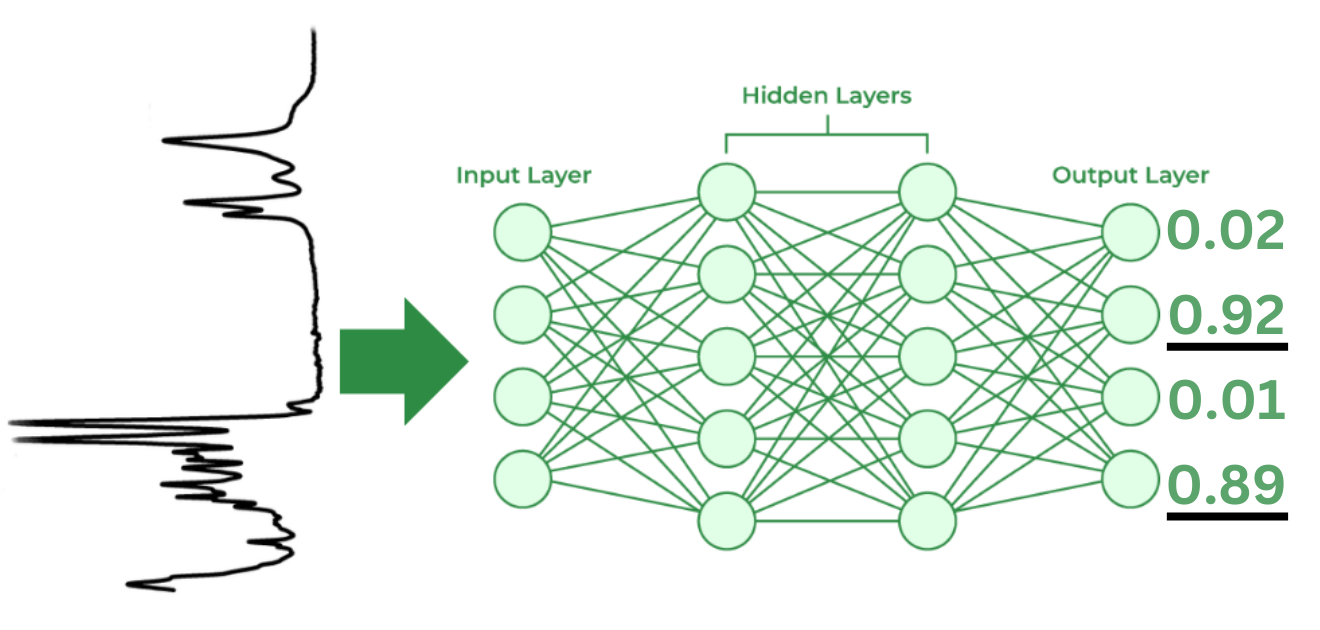
\includegraphics[width=0.8\textwidth]{Images/N2.png}
    \caption{Classificacao de funcoes organicas}
    \label{fig:ir_spectrum}
\end{figure}


No problema de classificação  de moléculas recebemos o espectro como input e criamos uma distribuição de probabilidades de ser cada molécula, que pode ser somado para 1, pois a amostra apenas pode ser uma molécula do dicionário. No entanto uma molécula pode conter mais de uma função orgânica, assim na classificação de funções orgânicas  o output final não soma para 1, mas sim cada neurônio na camada final representa uma  independente de 0 a 1 desta função orgânica está presente na molécula. 


\section{Dados}

...


\section{Implementação}
...

\section{Conclusão}
...



% Comment out the bibliography-related commands if you don't have a .bib file
% \bibliographystyle{plain}
% \bibliography{references}

\end{document}
